\chapter{System design and implementation}
\label{chapter:system-design}

This chapter presents the entire work of the author. The work is split into three parts in the attempt to combine deep neural networks with Q-Learning. The game chosen for the  experiment is the Tower of Hanoi due to its simplicity and also, due to the static environment. Afterwards, the values obtained through Q-Learning have been used to train a deep convolution network combined with the generated frames. Finally, our attempt is to combine the Q-learning algorithm with convolution networks.



\section{Q-Learning}
\label{sec:ql}
In this section we attempt to find the optimal policy for playing the Tower of Hanoi game. The algorithm starts with a pool of actions initialized with {UP, DOWN, LEFT, RIGHT} and a table Q containing the values for every (state,action) pair. 

The discount factor $\gamma$ is set to 0.95, the future rewards being taken into account when updating the action-value function. The learning rate $\alpha$ is chosen at 0.1, thus the algorithm can converge to an optimal policy. 

The exploration vs. exploitation problem is solved by using a variable $\epsilon$ which is initialized with 1 (1 is used when choosing only random actions and 0 when the action that can maximize the score is chosen). In order to make the current policy converge to the optimal policy the number of iterations used is set to 11 and the number of episodes per iteration set to 1000. After each iteration is finished, $\epsilon$ it is decreased with 0.1 until it will take the value 0. This method has been used to let the agent explore using random actions in the first iteration, afterwards exploiting the values learned in the last iterations.

After all the iterations are finished, the algorithm generates a dataset. For each value stored in Q-table, it generates the frame from each coded state.

On the next page, a pseudocode of Q-Learning is presented, which is an adaptation after the algorithm found in Norvig's book{\cite{norvig}}. The algorithm tries to estimate an optimal action-value function using the $\epsilon$-greedy policy, more exactly, it chooses a random action with probability $\epsilon$ and chooses the optimum action with probability 1-$\epsilon$.
\newpage
\begin{algorithm}
	\floatname{algorithm}{Algorithm}
	\caption{Q-Network} \label{alg-code}
	\begin{algorithmic}[1]
		\State set size of Q to with no_states x no_action and initialize it
		\State choose $\epsilon$ between (0,1)
		\State let \textbf{s} be the current state of the game
		\State let \textbf{actions} be a pool with {$a_1$,$a_2$,...,$a_n$}
		\While{game not over}
			\State r = random number between (0,1)
			\If{r < $\epsilon$}
				\State $a_t$ = random action
			\Else
				\State $a_t$ = $argmax_a$ Q(s, a)
			\EndIf
			
			\State $s^\prime$, r = apply_action(a, s)
			\State Q(s,a) = Q(s,a) + $\alpha\cdot$(r + $\gamma\cdot \max_a Q(s^\prime,a^\prime)-Q(s,a)$)
		\EndWhile
	\end{algorithmic}
\end{algorithm}

\section{Convolutional Neural Networks}
This section comes with an attempt to discuss various architecture models that could be suitable for our problem. To see if the network fits the main theme of this paper, one must provide proof that the network model can be generalized and is not hitting the ``high variance problem''. In order to come with a scientific proof or at least an empirical one, several experiments have been made.

\subsection{Regression with deep-learning and complex model}
The model proposed by Yann Lecun et al.\cite{energy-based} was slightly modified in order to map our problem. For the purpose of keeping things clear and well-separated every discussion about a network should be split into the next subjects: preprocessing data, chosen model for the network, loss function, training and testing.

For the first attempt, a model used in face detection and pose estimation has been chosen because good results in learning features relevant for object recognition have been promised. Also, it is possible for this model to be applied over large images.

\subsubsection{Data}

In this section \ref{sec:ql}, we generated a dataset of 160 images with 4 labels for each one (Tower of Hanoi has 160 states and offers 4 possible actions). In this section we try to build a convolutional neural network capable of predicting those values from images. This is made for the sake of bringing strong proof that our network model is capable of learning features from the dataset and not leading, instead, to a ``dead'' network which is ``overlearning'' and cannot be used on new samples.

First step was to resolve the problem of the small number of samples (160) from the dataset. This has been solved by generating 64 other datasets (to achieve approximately 10,000 samples) from the original one with noise added or color changed. In this way we can ensure that the network is capable of learning features dependent on size in this case.

The next figure(\ref{fig:155}) represents a state of the game and the next ones(\ref{fig:states}) represent altered images with noise added and color changed.

\begin{figure}[h]
	\begin{center}
		\frame{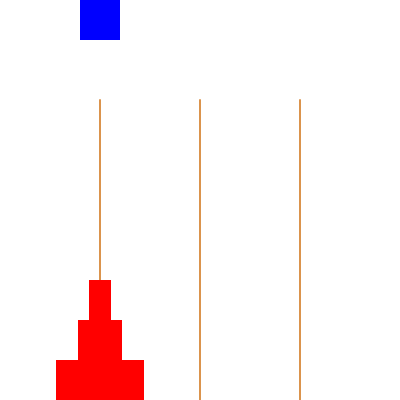
\includegraphics[width=130px,height=130px]{src/img/system-design/155}}
		\caption{Initial state of the game ``Tower of Hanoi''} \label{fig:155}
    \end{center}
\end{figure}

\begin{figure}[h]
	\begin{center}
		\frame{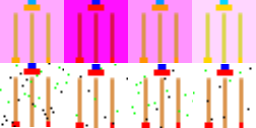
\includegraphics[width=253px,height=126px]{src/img/system-design/states}}
		\caption{Altered dataset} \label{fig:states}
    \end{center}
\end{figure}


For the preprocessing data various problems have been encountered. First of all, there is a large discussion on the RGB vs. YUV topic. This paper implements the YUV transformation based on the assumption that luminance should be separated from chrominance. If features dependent on color should be learned, then the neurons connected with the chrominance pixels will be activated, otherwise the neurons connected with luminance pixels will be activated. Both types of channels are kept in the attempt to make an algorithm that could make a better generalization.  Also, the YUV color is much closer to the human vision than RGB. 

The decision not to work with the 1-channel colors spaces such as grayscale is well-founded. There are games where size should not be a feature to be learned and in this cases we are interested in learning features dependent on color.

The next step was to normalize the images for aligning the range of pixel intensity values to a normal distribution. In other words, the histogram of the images are stretched and the contrast is improved in order to get sharp edges.

The normalization of the images implies computing the mean and the standard deviation. These values are computed for the training dataset of each channel. Then, we add the mean and divide it by standard deviation. This operation is applied on each channel from both datasets (train and test).

Another way to improve the contrast is using a gaussian matrix which follows a gaussian distribution, as it is clear from its name. The gaussian distribution states that average things should occur frequently and extreme things should occur rarely. The gaussian matrix will slide all over the image and will modify the pixel values such that the pixels from the middle of the neighbourhood will be more important than the pixel values from the edge of the gaussian matrix. If the edge pixel values have a zero importance than the resulting image will be identical to the initial image.

On the other hand, labels also need to be processed. Because of the formula for estimating the action-value function (Q) different ranges of values were generated. For example, if we have to do regression on values as 0,..., 100 there would not be a problem because the delta range is $10^2$, but the values generated follow a delta range of $10^5$. This can cause instability in the network. These being said, the paper proposes to bring the values to the same range using a logarithmic function and of course, to normalize them to follow the normal distribution.

Data was also shuffled to avoid having consecutive states of the game.

\subsubsection{Model}

The model used for training the convolutional neural network is the model presented in the next paper: ``Synergistic Face Detection and Pose Estimation with Energy-Based Models''\cite{energy-based} with some modifications such that the model becomes suitable for our network.

The model follows another model called LeNet-5 proposed by Yann LeCun et al. which was used in document recognition\cite{basedlearning} for training a network that could recognize noisy handwritten characters. The results obtained by the network state that the error rate is small, under 1$\%$ which is extremely satisfying. Trained on noisy handwritten characters draws attention to one important aspect: if the model is capable of generalizing even in heavy conditions, why could it not be used in combination with Q-learning for playing games.

In the next figure(\ref{fig:myarch}) we can see how the network suggested in this article looks. 

\begin{figure}[h]
	\begin{center}
		\includegraphics[width=410px,height=87px]{src/img/system-design/myarch}
		\caption{ConvNet Architecture} \label{fig:myarch}
    \end{center}
\end{figure}

The network is composed of three layers. Each layer applies kernel convolutions and samples on the data. After each layer we use the hyperbolic tangent as the layer activation function. As discussed in the paper ``Efficient Backprop'' by Yann LeCun et al., the motivation for using the hyperbolic tanh is similar to the one of normalizing data. The mean of the output data tends to be closer to zero, thus it is less likely to cause instabilities in the network derivatives when used in combination with back-propagation.

After the final layer, the sigmoid activation function has been used because the labels are normalized by scaling between 0 and 1.

The input layer consists of no_features x no_pixels_width x no_pixels_height neurons and the output layer has 4 neurons because only 4 actions are needed to play Tower of Hanoi.

The last layers are fully connected and for hidden layers the Spatial Convolution and Sub Sampling have been used. In the appendix \ref{appendix:model} the implementation in Torch7 can be found.

\subsubsection{Loss function}
For computing the error, Mean Squared Error was used. Being a task of regression, and not a task of classification the MSE is most appropriate for use.
\begin{equation}
loss(target,output) = \frac{1}{no_{samples}}\cdot\displaystyle\sum_{i=1}^{no_{samples}}\cdot((output^{(i)}) - target^{(i)})^2
\end{equation}


\subsection{Classification with deep-learning and complex model}

Because the last results for doing regression with convolutional networks did not match the author's expectations, another option have been provided. What if we try to learn the same results using a clasificator? All in all, we try to predict the action for every state.

Firstly, we change the architecture from LeNet-5 with the one used for training on Google Street View House Numbers proposed by Yuval Netzer et al. in the ``Reading Digits in Natural Images with Unsupervised Feature Learning''\cite{svhn} paper. The dataset used by them is very similar with the MNIST database (Yann Lecun)\footnote{\url{http://yann.lecun.com/exdb/mnist/}} except for the fact, that SVHN\footnote{\url{http://ufldl.stanford.edu/housenumbers/}} provides natural scene images.

\subsubsection{Data}
For predicting classes we need to transform continuous values to labels and for each state of the dataset we choose the label (\'up\' = 1, \'down\' = 2, \'left\' = 3, \'right\' = 4) according the maximum value. If the value corresponding to the \`up\`-action is the biggest, then we choose label 1.
Like the previous model architecture, the data is converted from RGB to YUV color space, to separate the luminance from chrominance. After this step they perform contrast normalization to sharpen edges and also, the normalization is performed.

\subsubsection{Model}
The model proposed for training the network is slightly different the the other one. The input remains the same, 3 channels and 32x32 size. The output is formed by four neurons corresponding for each action. The hidden layer activation functions used for the model is also tanh. The network is composed by two convolution layer and two pooling layers.

\subsubsection{Loss function}
For computing the error, Log Soft Max was used. Being a task of classification, and not a task of regression we need our network to map categorical information (discrete values variables) on continuous normalized data.

\begin{equation}
loss(x^{(i)}) = \log {\frac{1}{\displaystyle\sum_{j} e^{x^{(j)}}\cdot e^{x^{(i)}}}}
\end{equation}

\subsection{Regression with deep-learning and simple model}


Both of the last experiments using convolutional neural networks did not lead to satisfactory results and that is the reason we propose another model. We found that sometimes RGB may lead to better improvements than YUV\cite{pipeline} so we passed the images to CNN into RGB color-space. Another preprocessing step was removing contrast normalization because it does not improve the results, leading to overfitting. The new model comes with two convolutions and two poolings. The output activation functions remain the same, tanh for hidden layers and sigmoid for the output layers in order to predict the values from Q-Learning which are between 0 and 1. We removed one fully connected layer and let 150 neurons on the last hidden layers. An implementation in Torch7 can be found in appendix \ref{appendix:good-model}.

\subsection{Q-Network}

In this section we discuss the implementation for Q-Network adapted to our needs. In the \ref{fig:qmodel} is given a graphical representation of the whole model. The experiment was done on Tower of Hanoi games as the other experiments were done. On the preprocessing step the image were rescaled to 32x32 and the input given to the Q-Network is keeping the RGB color space. For the model we used the simple model discussed in the last section. This time we started with two networks: the action-value network Q and the action-value target network $Q^-$. The loss function is the same, MSE.

Then, we train the network as it follows: we start with a $\epsilon$-probability of 100\% in choosing a random action and 0\% for choosing the best action. After every 9 episodes we update the $\epsilon$-probability by decreasing it with 10\%. After we choose the action we observe the new state and the reward. We give the new sample to the $Q^-$ network and update the output corresponding to the action we have made with the reward if the episode had finished or with the q-learning equations. We compute the loss between Q and $Q^-$ and propagate loss derivative through Q. Every 100 steps we update the weights of $Q^-$ with the ones of Q.


\begin{figure}[h]
	\begin{center}
		\frame{\includegraphics[width=321px,height=210px]{src/img/system-design/qmodel}}
		\caption{Q-Network} \label{fig:qmodel}
    \end{center}
\end{figure}

